\documentclass[conference]{IEEEtran}


\usepackage[table]{xcolor}
\usepackage{cite}
\usepackage{url}
\usepackage[pdftex]{graphicx}


\begin{document}


\title{Predicting Mutation Score Using Source Code\\and Test Suite Metrics}


\author{\IEEEauthorblockN{Kevin Jalbert, Jeremy S. Bradbury}
\IEEEauthorblockA{Software Quality Research Group\\
University of Ontario Institute of Technology\\
Oshawa, Ontario, Canada\\
\{kevin.jalbert, jeremy.bradbury\}@uoit.ca}}


\maketitle


\begin{abstract}
Traditionally mutation testing has been used to evaluate the effectiveness of test suites and provide confidence in the testing process. Mutation testing involves the creation of many versions of a program -- each with a single syntactic fault. A test suite is evaluated against these program versions (mutants) in order to determine the percentage of mutants a test suite is able to identify (mutation score). A major drawback of mutation testing is that even a small program may yield thousands of mutants and can potentially make the process cost prohibitive. To improve the performance and reduce the cost of mutation testing, we propose a machine learning approach to predict the mutation score based on source code and test suite metrics.
\end{abstract}


\IEEEpeerreviewmaketitle


\section{Introduction}
\label{sec:introduction}
Mutation testing traditionally has been used as a coverage technique to evaluate the effectiveness of test suites and provide confidence in the testing process~\cite{DLS78, OAL06, JH10}. For over 30 years, mutation has been applied to software written in programming languages including C~\cite{DM96, JH08}, Fortran~\cite{KO91}, Java~\cite{MKO02, BCD06} and more. Furthermore, mutation testing has also been applied to other non-programming artifacts such as formal specification languages~\cite{ABM98} and spreadsheets~\cite{AE09}.

Mutation testing uses a set of \emph{mutation operators} to generate faulty versions of a program called \emph{mutants}. Mutation operators are created based on an existing fault taxonomy and each operator usually corresponds to a specific type of fault. A mutant is identical to the original program except that it contains a single mutation -- ``\emph{a single syntactic change that is made to a program statement.}''~\cite{KO91}. A test suite is evaluated against a set of mutants to determine the \emph{mutation score}. The mutation score is defined as the percentage of non-equivalent mutants that are detected (\emph{killed}) by a test suite. The better a test suite, the more mutants will be killed and thus the higher the mutation score.

A major drawback of mutation testing is that even a small program may yield hundreds or thousands of mutants potentially making the process cost prohibitive in comparison to other coverage metrics such as statement or branch coverage. Several approaches have been proposed in the literature to improve mutation testing performance and scalability~\cite{OU00}:

\begin{itemize}
  \item \textbf{``Do fewer'' approach:} this category of optimizations aim to decrease the computational cost of mutation testing by reducing the number of mutants that a test suite is evaluated against. The most popular example from this category is selective mutation -- the use of a subset of mutation operators that have been empirically shown to be as effective as using an entire set of operators~\cite{OLR+96}. Another example of a ``do fewer'' approach is to randomly sample mutants~\cite{Won93}.

  \item \textbf{``Do smarter'' approach:} this category of optimizations aim to decrease the cost of mutation testing by improving the actual mutation testing technique. For example, weak mutation \emph{``...is an approximation technique that compares the internal states of mutant and original program immediately after execution of the mutated portion of the code (instead of comparing the program output)''}~\cite{OU00}.

  \item \textbf{``Do faster'' approach:} this category of optimizations aim to reduce the cost of mutation testing by focusing on performance. For example, one ``do faster'' approach improves compilation time using schema-based mutation -- \emph{``...encodes all mutations into one source level program...''}~\cite{OU00}.
\end{itemize}

As an alternative to the above techniques, we propose a ``do fewer and smarter'' technique for mutation testing at a unit level.  When mutation testing is used for the creation or improvement of a test suite,  the test suite will often have to be applied to the mutants in an iterative fashion as tests are added, removed and modified. Furthermore, the effects on the mutation score after each iteration have to be observed. We propose to replace at least some of these intermediate test suite evaluations on mutants with mutation score prediction and thus decrease the number of mutants that have to be evaluated using a test suite. Our proposed approach uses machine learning to predict the mutation score based on a combination of source code and test suite metrics of the code unit under test.

In the Section~\ref{sec:background} we describe the machine learning technique, the mutation testing tool and the metrics gathering tools used in our research. In Section~\ref{sec:approach} we describe our overall approach to mutant score prediction. We also discuss the integration of the tools described in the previous section, into our approach. In Section~\ref{sec:case_study} we apply our approach to an open source project and discuss the effectiveness of our prediction based on this preliminary evaluation. Finally, in Sections~\ref{sec:related_work}~\&~\ref{sec:conclusions_future_work} we discuss related work, conclusions, and future work.


\section{Background}
\label{sec:background}
In this section we describe the background techniques and tools used in our research. In particular, we discuss LIBSVM, support vector machine library, Javalanche, a mutation testing tool, the Eclipse Metrics Plugin, used for gathering source code metrics, and EMMA, used for acquiring test suite metrics.


\subsection{LIBSVM -- a library for support vector machines}
\label{subsec:libsvm}
A support vector machine (SVM) is an example of a linear discrimination machine learning technique and assumes that ``...\emph{instances of a class are linearly separable from instances of other classes}''~\cite{ALP04}. In other words, a SVM learns the linear discriminant of a set of data. SVMs are capable of learning how a set of features inform the classification of a data item. It can also be trained on known data items (in which the features and category are present), and then used to predict the category of  unknown data items (in which only the features are present).

Traditionally, SVMs have been used for two-group classification problems~\cite{CV95} but have also been generalized to \emph{n}-group classification problems. In a two-group classification problem this approach identifies an optimal separating hyperplane that divides the set of data into two groups based on a set of support vectors (i.e., features). In other words, the goal is to maximize the distance from the closest data points on both sides of the hyperplane to the hyperplane itself~\cite{ALP04}.

In our research we use LIBSVM\footnote{LIBSVM version 3.11}, a SVM library capable of solving \emph{n}-group classification problems~\cite{CL11}. LIBSVM was chosen because it provides a command-line interface that could be easily integrated with the other tools used in our approach.


\subsection{Javalanche -- a mutation testing tool for Java}
\label{subsec:javalanche}
Mutation testing has previously been described in Section~\ref{sec:introduction}. In our research we use Javalanche\footnote{Javalanche version 0.4}, a mutation testing tool for Java~\cite{SZ09} that applies a subset of the method-level mutation operators to source code. Method-level operators are the most common set of mutation operators applied to procedural programming languages and each method-level mutation defines a syntactic change to an operator, operand or statement in a program. The subset of the method-level operators used by Javalanche are know as the selective method-level mutation operators (see Table~\ref{tab:mutation_operators}). These operators have been empirically shown to be as effective as using the entire set of method-level operators~\cite{OLR+96}.

\begin{table}[!t]
  \centering
  \rowcolors{2}{gray!30}{gray!20}
  \begin{tabular}{|l|l|}
    \hline
    \rowcolor[RGB]{169,196,223}
    \textbf{Name} & \textbf{Description} \\
    \hline REPLACE\_CONSTANT & Replace a constant \\
    \hline NEGATE\_JUMP & Negate jump condition \\
    \hline ARITHMETIC\_REPLACE & Replace arithmetic operator \\
    \hline REMOVE\_CALL & Remove method call \\
    \hline REPLACE\_VARIABLE & Replace variable reference\\
    \hline ABSOLUTE\_VALUE & Insert absolute value of a variable \\
    \hline UNARY\_OPERATOR & Insert unary operator \\
    \hline
  \end{tabular}
  \caption{The set of selective method-level mutation operators used in Javalanche~\cite{ OLR+96}}
  \label{tab:mutation_operators}
\end{table}


\subsection{Eclipse Metrics Plugin - a source code metrics tool}
\label{subsec:Metrics}
Source code metrics measure knowledge of a project's source code through the use of code analysis~\cite{SCE05,McCa76,Kan02}. Source code metrics give insight into various aspects of the source code including it's complexity, size, coupling, cohesion as well as object-oriented attributes~\cite{Hend95}.

In our research, we use the Eclipse Metrics Plugin\footnote{Eclipse Metrics Plugin version 1.3.8.20100730-001} to acquire source code metrics of the methods and classes under test. We selected this tool as it provides a comprehensive set of metrics for Java programs. We do not use all of the metrics reported by the Eclipse Metrics Plugin but instead we only use the metrics at the method and class level (see Table~\ref{tab:source_code_metrics})~\cite{Metrics}.

\begin{table}[!t]
  \centering
  \rowcolors{2}{gray!30}{gray!20}
  \begin{tabular}{|l|l|l|}
    \hline
    \rowcolor[RGB]{169,196,223}
    \textbf{Abbreviation} & \textbf{Description} & \textbf{Scope} \\
    \hline MLOC & Method lines of code &  Method \\
    \hline NBD & Nested block depth &  Method \\
    \hline VG & McCabe cyclomatic complexity &  Method \\
    \hline PAR & Number of parameters &  Method \\
    \hline NORM & Number of overridden methods &  Class \\
    \hline NOF & Number of attributes &  Class \\
    \hline NSC]& Number of children &  Class \\
    \hline DIT & Depth of inheritance tree &  Class \\
    \hline LCOM & Lack of cohesion of methods &  Class \\
    \hline NSM & Number of static methods &  Class \\
    \hline NOM & Number of methods &  Class \\
    \hline SIX & Specialization index &  Class \\
    \hline WMC & Weighted method per class &  Class \\
    \hline NSF & Number of static attributes &  Class \\
    \hline
  \end{tabular}
  \caption{The set of source code metrics measured by the Eclipse Metrics Plugin~\cite{Metrics} that are used in our research.}
  \label{tab:source_code_metrics}
\end{table}


\subsection{EMMA - a test suite coverage tool}
\label{subsec:emma}
Test suite metrics can be gathered using similar technique to those used in the gathering of source code metrics. In fact, since we focus on JUnit test cases (which are Java classes) we can actually use the Eclipse Metrics Plugin to gather some of the test suite metrics. To gather other test suite metrics we use the tool EMMA\footnote{EMMA version 2.0.5312} which is capable of determining the statement and basic block coverage of a test suite~\cite{EMMA}. We include coverage metrics because they are important indicators of test suite effectiveness. 


\section{Approach}
\label{sec:approach}
We now describe our approach to determining the mutation score of a unit under test based on source code and test suite metrics. In Section~\ref{subsec:training} we outline the process for collecting our initial data and training the SVM (see Figure~\ref{fig:process}) and in Section~\ref{subsec:prediction} we describe how to use the SVM for prediction and cross-validation.

\begin{figure*}[!t]
  \centering
  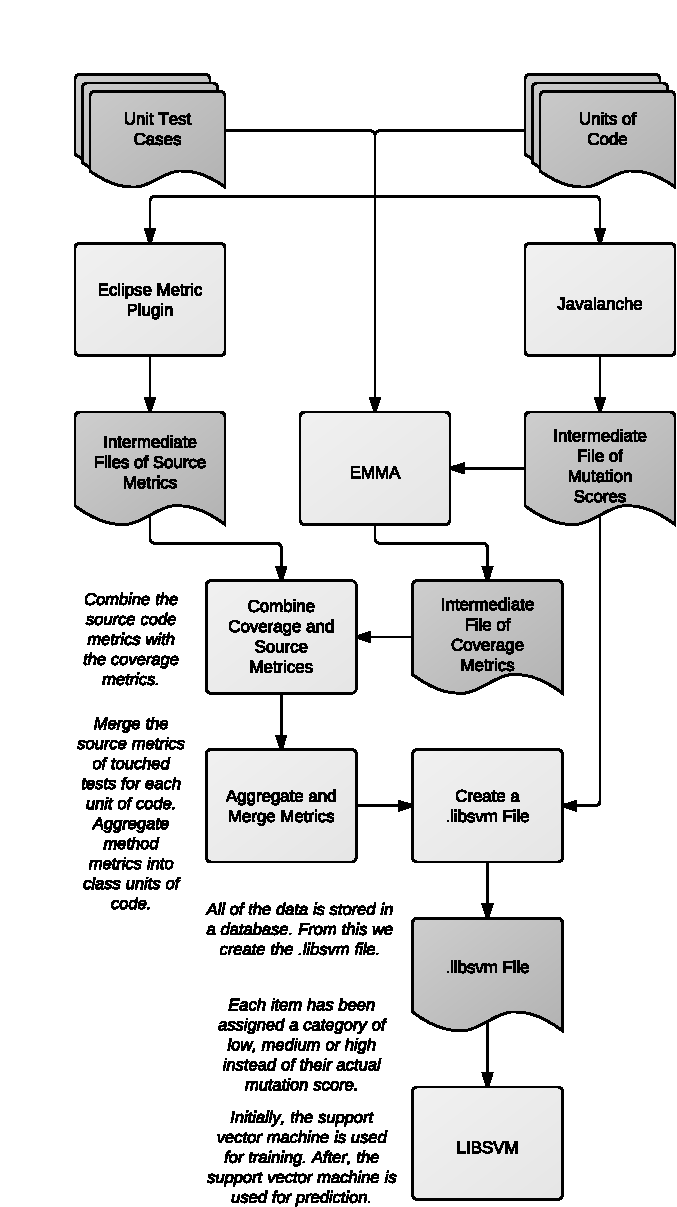
\includegraphics[width=13cm]{figures/process.pdf}
  \caption{Our training process -- using source code and test suite metrics to determine mutation score for a unit under test.}
  \label{fig:process}
  \vspace{2mm}
  \hrule
\end{figure*}


\subsection{Training}
\label{subsec:training}
The input that our training process requires is a set of units of code in which each unit of code has a corresponding set of unit test cases. Both the units under test and test cases (i.e., JUnit tests) are Java source files.

The first step of our process is to collect the two types of data required to train the SVM:

\begin{enumerate}
  \item \textbf{Category Data:} Javalanche is used to generate the mutants of all units in the project under test. In addition to mutant generation, Javalanche also performs the mutation testing by executing the required tests for each mutant, although it currently does not exclude equivalent mutants from the analysis. For our research, we added a new analyzer component to Javalanche that outputs an intermediate text file of mutation scores of the covered units (methods and classes). This intermediate text file also contains a list of every test that was executed for each method.

  \item \textbf{Feature Data:} The feature data is comprised of the source code and test suite metrics. To collect the source code metrics of the project we use the Eclipse Metrics Plugin. We collect metrics not only of the units of code under test, but also the unit test cases. After the metrics are collected they are exported to intermediate text files of source code and test suite metrics for methods and classes.

  To collect the additional test suite specific metrics, we acquire the statement coverage and basic block coverage of each unit under test using EMMA. We use EMMA to determine the  coverage of each method by only examining the set of executed tests that Javalanche reported. This information is also exported to an intermediate text file containing the test suite coverage metrics.
\end{enumerate}

Next, we combine all the data contained in the intermediate text files into a database. Since we are interested in both method and class units under test we are not only interested in method-level metrics but also class-level metrics. Therefore, for a given class we aggregate and merge metrics from the each contained methods to generate the class metrics.

Next, we create a .libsvm file containing the category and feature data from the database. Instead of predicting a specific mutation score percentage, we categorize all mutation scores as \textit{low, medium, high} which reduces the mutation score prediction to a three-group classification problem. The ranges are determined based on the distribution of the mutation scores in our training data (further explained in Section~\ref{subsec:results}). Finally, the .libsvm file is passed into LIBSVM to complete the training process.


\subsection{Prediction}
\label{subsec:prediction}
Once we have trained the SVM, we can then use the SVM for prediction. We can predict the category of an unknown unit of code by first extracting the source code and test suite metrics. The extracted features are then passed into the SVM which will then be assigned a category of \textit{low, medium, high} for the mutation score.  Currently, our approach only predicts mutation scores within a project. That is, the training and prediction data both come from the same project repository.

It is also possible to perform cross-validation to assess the accuracy of the approach for a given set of training data. Typically cross-validation is used when there is not a lot of data available for training and prediction. Cross-validation splits up the provided dataset into \emph{n} equal-sized partitions and the SVM internally train on $\emph{n}-1$ sets and predict the last. This process is repeated \emph{n} times where a different partition is selected for prediction each time. Finally all the individual prediction accuracies are tallied and averaged for a cross-validation accuracy of \emph{n}-folds (i.e., a 10-fold cross-validation is common).


\section{Case Study: JGAP}
\label{sec:case_study}
We will now discuss the prediction results of our mutation score predictor using an open source Java project.

The project, JGAP\footnote{JGAP version 3.6.1} a genetic algorithm and genetic programming framework for Java, was selected due to its comprehensive JUnit testing suite~\cite{JGAP}. We decided to use an open source project that is large enough to contain many mutants, as well as a mature test suite. Basic source code metrics for JGAP are provided in Table~\ref{tab:jgap_source_stats}. 
JGAP contains 1348\footnote{JGAP has 1412 JUnit test cases in total, however a small percentage of the tests caused errors in the Javalanche tool and were removed.} usable JUnit test cases. For JGAP Javalanche generated 30022 mutants using the method-level mutation operators (see Table~\ref{tab:mutation_operators}) of which only 16982 were actually covered by JGAP's test suite. We only considered the set of covered mutations in our approach as the mutations not covered contained no associated test cases. Considering only the covered mutants JGAP's test suite killed 12631 mutants resulting in an overall mutation score of 74.38\% (see Table~\ref{tab:jgap_mutation_stats} for more detail).

\begin{table}[!t]
  \centering
  \rowcolors{2}{gray!30}{gray!20}
  \begin{tabular}{|l|r|r|}
    \hline
    \rowcolor[RGB]{169,196,223}
    \textbf{JGAP Source Artifacts} & \textbf{\# in Source} & \textbf{\# in Test} \\
    \hline Classes & 415 & 180 \\
    \hline Methods & 3017 & 1626 \\
    \hline LOC & 28975 & 19556 \\
    \hline JUnit Test Cases & -- & 1412\footnotemark[6] \\
    \hline
  \end{tabular}
  \caption{The amount of classes, methods, lines of code (LOC), and JUnit test cases in the JGAP repository}
  \label{tab:jgap_source_stats}
\end{table}

\begin{table}[!t]
  \centering
  \rowcolors{2}{gray!30}{gray!20}
  \begin{tabular}{|l|r|}
    \hline
    \rowcolor[RGB]{169,196,223}
    \textbf{Javalanche Artifacts} & \textbf{\# of Occurrences} \\
    \hline Valid JUnit Test Cases & 1348\footnotemark[6] \\
    \hline Generated Mutants & 30022 \\
    \hline Covered Mutants & 16982 \\
    \hline Killed Mutants & 12631 \\
    \hline Overall Mutation Score & 74.38\% \\
    \hline
  \end{tabular}
  \caption{Mutation results of JGAP. The valid test cases are those which successfully ran in Javalanche. The killed mutants and overall mutation score are using the covered mutants.}
  \label{tab:jgap_mutation_stats}
\end{table}


\subsection{Results}
\label{subsec:results}
We first decided to view the distribution of JGAP's mutation scores, which are shown in Figure~\ref{fig:mutation_class_distributions} \& \ref{fig:mutation_method_distributions}. It is clearly obvious that the distribution for both classes and methods are more heavily dense for high mutation scores. Of the 547 method data and 136 class data we collected we found that 19.85\% of the class data and 29.80\% of the method data have a mutation score $\le$ 1\% or $\ge$ 99\%.

\begin{figure}[!t]
  \centering
  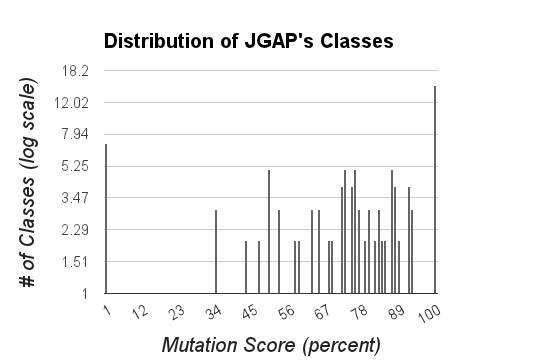
\includegraphics[width=10cm]{figures/class_distribution.png} 
  \caption{The mutation score distribution of JGAP's classes that can be used for training.}
  \label{fig:mutation_class_distributions}
  \vspace{2mm}
  \hrule
\end{figure}

\begin{figure}[!t]
  \centering
  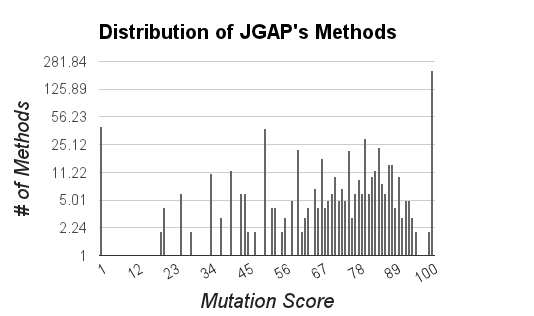
\includegraphics[width=10cm]{figures/method_distribution.png}
  \caption{The mutation score distribution of JGAP's methods that can be used for training.}
  \label{fig:mutation_method_distributions}
  \vspace{2mm}
  \hrule
\end{figure}

As mentioned in Section~\ref{subsec:training} we categorize the collected data into three groups of \textit{low, medium, high} based on their mutation scores. Ideally we would like to have sufficient data coverage for the complete range of mutation scores, such that we can train the SVM using simple categories such as 0\%--33\% (\textit{low}), 33\%-66\% (\textit{medium)} and 66\%-100\% (\textit{high}). Given our situation of not being able to split up the collected data easily across the mutation scores we instead decided to categorize our data such that one third of our data will fall into each category. This results in varying mutation score ranges for each category for class- and method-level data as shown in Table~\ref{tab:results_details}.

\begin{table}[!t]
  \centering
  \rowcolors{2}{gray!30}{gray!20}
  \begin{tabular}{|l|r|r|}
    \hline
    \rowcolor[RGB]{169,196,223}
    \textbf{Category} & \textbf{Class Mutation Score} & \textbf{Method Mutation Score} \\
    \hline low & 0\% -- 61\% & 0\% -- 75\% \\
    \hline medium & 61\% -- 84\% & 75\% -- 90\% \\
    \hline high & 84\% -- 100\% & 90\% -- 100\% \\
    \hline
  \end{tabular}
  \caption{The mutation score ranges that equally partition the datasets into three categories. These ranges are for the JGAP project and are determined by the 547 collected methods and 136 collect classes.}
  \label{tab:results_details}
\end{table}


To evaluate our results we decided to use a 10-fold cross-validation of our datasets due to the small amount of data acquired from this experiment. Our achieved accuracy for JGAP using cross-validation was 49.26\% for class-level mutation scores and 48.08\% for method-level mutation scores. It is also worth mentioning that our achieved accuracy outperforms random (which has an accuracy of 33.33\% given our category distributions) by at least 14.75\%. A further analysis of the acquired metrics used as the feature set in LIBSVM would prove useful in understanding the relevant and important metrics in mutation score prediction.


\section{Related Work}
\label{sec:related_work}
The use of software metrics to locate faults in source code has been well researched. For example, Koru et al. utilized static software measure along with defect data at the class level to predict bugs using machine learning~\cite{KL05}. Similarly, Gyimothy et al. used object-oriented metrics with logistic regression and machine learning techniques to identify faulty classes in open source software~\cite{GFS05}. Finally, design level metrics were used with a linear prediction model to determine the estimated maintainability and error prone modules of large software systems~\cite{MKPS00}. Our work is unique in comparison to these previous works since we not only use source code metrics but we also use test suite metrics to enhance our predication capabilities.


\section{Conclusions \& Future Work}
\label{sec:conclusions_future_work}
Our technique for predicting mutation score using source code and test suite metrics achieved an accuracy of 49.26\% and 48.08\% for classes and methods respectively -- outperforming random. These results have not been optimized and we believe that with further enhancements and a more tailored feature set we may be able to increase our prediction accuracy. 

In the future, we plan to evaluate more open source projects using our prediction technique to better assess the prediction accuracy. Also, we would like to consider projects with more mutation scores to explore the variation in prediction accuracy between strong and weak test suites. 

Currently we have applied our predictive technique to a single open source project -- JGAP. Another future direction we plan to investigate is whether cross-project models are valid for mutation score prediction. 


\bibliographystyle{IEEEtran}
\bibliography{references}


\end{document}
